%% This work may be distributed and/or modified under the
%% conditions of the LaTeX Project Public License, either version 1.3 of this license or (at your option) any later version.
%%
%% This work has the LPPL maintenance status `maintained'.
%%
%% INÍCIO DAS CUSTOMIZAÇÕES PARA A UNIVERSIDADE FEDERAL DE OURO PRETO

%% 10.09.2026 19h56 Danny Tonidandel
%% 	-	ALtera padrão para de cores oficiais da UFOP

%% 04.09.2026 19h56 Danny Tonidandel
%% Atualização normas pelo Comitê Brasileiro de Informação e Documentação da ABNT:
%% 	-	ALtera elementos de capa e folha de rosto 
%% 	-	Altera rótulos de gênero para orientador ou orientadora
%% 	-	Altera cor das urls e hyperlinks
%% 	-	Insere texto do tutorial em todos os capítulos/seções
%% 	-	Altera estrutura de capítulos e seções
%%	-	Trabalhos acadêmicos (ABNT NBR 14724/4. ed.: 16 dez. 2024); 
%% 	-	Citações em documentos (ABNT NBR 10520/2. ed.: 19 jul. 2025
%% 	-	Referências (ABNT NBR 6023/3. ed.: 21 maio 2025).
%% 	- 	Altera posições de legendas e fontes
%% 	-	Insere ambiente para realce de códigos
%% 	-	Insere ambiente para realce de texto (caixas)
%% 	-	Insere tópicos sobre a utilzação de IA na pesquisa acadêmcia

%% 10.09.2025 Danny Tonidandel

%% Altera padrão de capa, folha de rosto e folha de aprovação. Remove título de seção dos cabeçalhos

%% 2025.6.23 16h09 Danny Tonidandel

%% Altera opções para compilação com diferentes compiladores

%% 2022.3.30 13h15 Danny Tonidandel
%% Altera as definições de capa, alterando  o comando, inserindo figuras próprias da Universidade e alterando a disposição dos elementos na contra-capa
%% Remove itens de abstract em francês
%% Altera disposição dos elementos na folha de aprovação
%% Altera o conteudo dos capítulos para um arquivo único.
%% Personalização do estilo biblatex-abnt para adequação à normaABNT 6023:2018
% Reseta contadores das notas de rodapé em cada capítulo
% Insere comandos para exibir uma caixa colorida de fundo cinza para notas explicativas, à escolha do autor

%% 2017.5.31 21h13 Danny Tonidandel
%% Altera nome de arquivo de logomarca
%% remove resumos em espanhol e italiano
%% Insere exemplos para elaboração de tabelas
%% Insere tabela de cronograma de atividades (para projeto de pesquisa)


%% FIM DAS CUSTOMIZAÇÕES PARA A UNIVERSIDADE FEDERAL DE OURO PRETO

%% Esse trabalho consiste nos arquivos
% template-abnt-ufop-escola-de-minas.tex
% referencias.bib

% --------------------------------------------
% abnTeX2: Modelo de trabalho Academico (tese de doutorado, dissertacao de 
% mestrado e trabalhos monográficos em geral) em conformidade com as normas
% ABNT
% ------------------------------------------------------------------------

\documentclass[
	% -- opções da classe memoir --
	12pt,				% tamanho da fonte 12
	openright,			% capítulos começam em pág ímpar (insere página vazia caso preciso)
	oneside,			% p/ impressão verso e anverso: twoside
	a4paper,			% tamanho do papel.
	% -- opções da classe abntex2 --
	%chapter=TITLE,		% títulos de capítulos convertidos em letras maiúsculas
	%section=TITLE,		% títulos de seções convertidos em letras maiúsculas
	%subsection=TITLE,	% títulos de subseções convertidos em letras maiúsculas
	%subsubsection=TITLE,% títulos de subsubseções convertidos em letras maiúsculas
	% -- opções do pacote babel --
	english,			% idioma adicional para hifenização
	brazil				% o último idioma é o principal do documento
	]{abntex2}

% --- Pacotes básicos
\usepackage{graphicx} 	% gráficos
\usepackage{graphbox} %  para alinhamento vertical  com 'align=c'
\usepackage{lscape} % figuras em paisagem
\usepackage[table,xcdraw]{xcolor} % tabelas
\graphicspath{{figuras/}} % pasta para figuras
\DeclareGraphicsExtensions{.pdf,.eps,.svg,.png,.jpg,.bmp} % extensões
\usepackage{caption} % para configrações em legendas


\usepackage{indentfirst} % para identação no primeiro parágrafo
\usepackage{booktabs}
\usepackage{microtype} 	% justificação
\usepackage{verbatim}

% Pacotes de escrita matemática
\usepackage{amsmath,amssymb,unicode-math}

% alterações nas margens 
\usepackage{geometry}

\usepackage{pdfpages} %  anexar pdf diretamente no documento
\usepackage{csquotes}


% Citações
\usepackage[backend=biber,
% configuracoes do estilo abnt
 style=abnt,
 citecount, % contar o número de citações
 justify, % alinhamento justificado
 noslsn,
 ]{biblatex}

% Arquivo de referências
\addbibresource{referencias.bib}



% Aparência do PDF - Cores oficiais da UFOP {https://www.ufop.br/logomarca/}

\definecolor{VinhoUFOP}{cmyk}{0.00, 1.00, 0.64, 0.33} 
\definecolor{CinzaUFOP}{cmyk}{0.67, 0.00, 0.00, 0.64} 

% Configuração dos links do PDF
\hypersetup{
	colorlinks=true,       % remove as caixas
	linkcolor=VinhoUFOP,   % links internos
	citecolor=CinzaUFOP,   % citações bibliográficas
	urlcolor=VinhoUFOP,    % urls
	filecolor=CinzaUFOP,    % links para arquivos
	pdftitle={\@title},
	pdfauthor={\@author},
	pdfsubject={\imprimirpreambulo},
	pdfcreator={UFOP com LaTeX}
}

% ---
% Personalização do estilo biblatex-abnt - Danny A. V. Tonidandel

% Adequa as urls de acordo com normas 6023:2018
\DeclareFieldFormat{url}{\bibstring{urlfrom}\addcolon\addspace \url{#1}}%
\DeclareFieldFormat{urldate}{\bibstring{urlseen}\addcolon\addspace #1}%

% Reseta contadores das notas de rodapé em cada capítulo
\makeatletter
\@addtoreset{footnote}{chapter}
\makeatother

% insere ambientes em ``caixas''
\usepackage{mdframed}

% Configura o mdframed para inserir uma caixa cinza de nome ``caixa{}''
\newcommand{\caixa}[1]{%
	\begin{mdframed}[
		linewidth=1.5pt,
		leftmargin=10pt,%
		rightmargin=10pt,%
		%backgroundcolor=gray!50
		linecolor=VinhoUFOP
	]{\small #1}
	\end{mdframed}
}

% pacote para inserção de código e realce de sintaxe
\usepackage{listings}

% Realce de sintaxe de código
\lstdefinelanguage{CustomLaTeX}{
	keywords={documentclass, usepackage, begin, end, section, subsection, footnote, subsubsection, paragraph, appendix, bibliography, bibliographystyle, cite, textcite, textbf, textit, texttt, emph,  width, textwidth, centering, includegraphics, caption, ref, bfseries, small, normalsize, label},
	sensitive=true,
	comment=[l]{\%},
	morestring=[b]",
	morestring=[b]'
}

\lstset{
	language=CustomLaTeX,
	backgroundcolor=\color{white},
	basicstyle=\ttfamily\footnotesize, % Fonte menor que no texto
	keywordstyle=\color{VinhoUFOP}\bfseries,
	commentstyle=\color{CinzaUFOP}\itshape,
	stringstyle=\color{VinhoUFOP},
	emph={figure, citacao, equation, eqnarray, frac, to, left, right, theta, int, pi, alpha, limits, infty, tanh, omega, ln, h, nonumber, lim}, 
	emphstyle=\color{CinzaUFOP},
	breaklines=true,
	frame=single,
	numbers=left,
	numberstyle=\tiny\color{CinzaUFOP},
	captionpos=t,       % sempre no topo
	showstringspaces=false,
	rulecolor=\color{VinhoUFOP},
	framerule=0.7pt,
	xrightmargin=10pt,
	xleftmargin=10pt
}

% Renomeia o ambiente lstlistings para "Código"
\renewcommand{\lstlistingname}{C{\'o}digo}


% DADOS PARA CAPA E FOLHA DE ROSTO

% Título e subtítulo
\titulo{
	Um Estudo sobre a Dinâmica de Sistemas Complexos \\ 
	{\normalsize Modelo ABNT e Tutorial para TCCs - DECAT-UFOP} \\ {\small \textcolor{VinhoUFOP}{v26.09b}}
	}

% Autoria
\autor{Maria da Cunha}

% Orientação
\orientador[Orientadora:]{Profa. Dra. Chiquinha Gonzaga}
\coorientador{Prof. Dr. Albert Einstein}

%Local e Data
\local{Ouro Preto}
\data{\the\year} 

% Instituição
\instituicao{Universidade Federal de Ouro Preto}
\tipotrabalho{Monografia de Graduação}

% Preambulo
\preambulo{
	Trabalho apresentado ao Colegiado do Curso de Engenharia de Controle e Automação da Universidade Federal de Ouro Preto como parte dos requisitos para a obtenção do Grau de Engenheiro(a) de Controle e Automação.
	}

\makeatother
% ---

% Espaçamentos entre linhas e parágrafos
\setlength{\parindent}{1.3cm} % Tamanho do parágrafo
\setlength{\parskip}{0.2cm} % Espaçamento entre parágrafos
\makeindex % compila o indice

\usepackage{fancyhdr} % cabecalho ``chique''

% Ambientes de Teoremas e definições
\newtheorem{algoritmo}{Algoritmo}
\newtheorem{definicao}{Definição}
\newtheorem{exemplo}{Exemplo}
\newtheorem{solucao}{Solução}
\newtheorem{teorema}{Teorema}
\newtheorem{demonstracao}{Demonstração}

% Início do documento
\begin{document} 

\frenchspacing % Retira espaço obsoleto

% Capa
\begin{capa}
		\newgeometry{margin=2.5cm}
		\thispagestyle{empty}
		\centering
		
\includegraphics[height=2.7cm, align=c]{logo-universidade.jpg}%
		\hfill
		\begin{tabular}{c} \Large \imprimirinstituicao \\ {\large Escola de Minas} \\ {\large Engenharia de Controle e Automação} \end{tabular}%
		\hfill
		
\includegraphics[height=2.7cm, align=c]{logo-unidade-2.jpg}
		\centering
		\vspace*{1.6cm}
		
		{\ABNTEXchapterfont \Large \imprimirautor}
		\vspace*{\fill}
		
		{\ABNTEXchapterfont\bfseries \huge \imprimirtitulo}
		
		\vspace*{\fill}
		\vspace*{\fill}
		{\Large\imprimirlocal} \\ 
		{\large \the\year}
		%{\large\imprimirlocal}, {\large \the\year}
		%\par
		\vspace*{1cm}
		%
		\clearpage % Finaliza a página atual
		% Restaura as margens padrão do documento
		\restoregeometry
\end{capa}

% Folha de rosto [OBRIGATÓRIO]
\begin{folhaderosto}
	\thispagestyle{empty}
	\centering
	\begin{center}
		\centering
		\vspace*{1cm}
		{\ABNTEXchapterfont\Large\imprimirautor}
		
		\vspace*{\fill}
		
		{\ABNTEXchapterfont\bfseries \huge \imprimirtitulo}
		
		\vspace*{\fill}	
		\hfill % Empurra o conteúdo para a direita
		\begin{minipage}{0.5\textwidth} 
			%{\ABNTEXfontereduzida \imprimirpreambulo}
			{\imprimirpreambulo} \\
			{\imprimirorientadorRotulo~\imprimirorientador}\\
			{\imprimircoorientadorRotulo~\imprimircoorientador}
		\end{minipage}
		\vspace*{\fill}			
		
		{\large\imprimirlocal} \\ 
		{\large \the\year}
		%\par
		\vspace*{1cm}
	\end{center}
\end{folhaderosto}

% Folha de aprovação - [OBRIGATÓRIO]
\begin{folhadeaprovacao}

\includepdf{folha-de-aprovacao.pdf}
\end{folhadeaprovacao}

% Agradecimentos [OPCIONAL]
\begin{agradecimentos}
\noindent Os agradecimentos [são opcionais, e] vem aqui...
\end{agradecimentos}

% Epígrafe - [Opcional]
\begin{epigrafe}
    \vspace*{\fill}
{\textsl{Sua epígrafe aqui.}}\\{---~Autor da epígrafe.}
\end{epigrafe}

% Resumo em português [OBRIGATÓRIO]
	\setlength{\absparsep}{18pt} % ajusta espaçamento
	\begin{resumo}
	 \noindent O resumo deve ressaltar o objetivo, o método, os resultados e as conclusões do documento. A ordem e a extensão
	 destes itens dependem do tipo de resumo (informativo ou indicativo) e do tratamento que cada item recebe no documento original. O resumo deve ser precedido da referência do documento, com exceção do resumo inserido no
	 próprio documento. (\ldots) As palavras-chave devem figurar logo abaixo do resumo, antecedidas da expressão Palavras-chave:, separadas entre si por
	 ponto e finalizadas também por ponto.
	
	 \textbf{Palavras-chaves}: latex. abntex. editoração de texto.
	\end{resumo}

% resumo em inglês ou outra língua [OBRIGATÓRIO LINGUA ESTRANGEIRA]
\begin{resumo}[Abstract]
	 \begin{otherlanguage*}{english}
	
	\noindent This is the english abstract.
	
	   \vspace{\onelineskip}
	
	   \noindent
	   \textbf{Key-words}: latex. abntex. text editoration.
	 \end{otherlanguage*}
\end{resumo}

% Lista de figuras [OPCIONAL]
\renewcommand{\listfigurename}{Lista de figuras} % altera nome
\pdfbookmark[0]{\listfigurename}{lof}
\listoffigures*
\cleardoublepage

% Lista de tabelas [OPCIONAL]
\pdfbookmark[0]{\listtablename}{lot}
\listoftables*
\cleardoublepage

% Lista de abreviaturas e siglas [OPCIONAL]
\begin{siglas}
  \item[UFOP] Universidade Federal de Ouro Preto
  \item[Automic Jr] Empresa Júnior do Curso de Engenharia de Controle e Automação
  \item[CAT490] Disciplina trabalho Final de Curso I
\end{siglas}

% Lista de símbolos [OPCIONAL]
\begin{simbolos}
  \item[$ \Gamma $] Letra grega Gama
  \item[$ \Lambda $] Lambda
  \item[$ \zeta $] Letra grega minúscula zeta
  \item[$ \in $] Pertence
\end{simbolos}

% Sumário [OBROGATÓRIO]
\pdfbookmark[0]{\contentsname}{toc}
\tableofcontents*
\cleardoublepage


% Reinicia contadores das notas
\makeatletter
\@addtoreset{footnote}{chapter}
\makeatother

% Parte textual
\textual

%% remove decoração cabecalhos
\fancypagestyle{plain}{%
	\fancyhf{} % limpa tudo
	\fancyhead[R]{\thepage} % número no topo à direita
	\renewcommand{\headrulewidth}{0pt} 
	\renewcommand{\footrulewidth}{0pt} 
}

\pagestyle{plain}


% -- seção primária - 
\chapter[Introdução]{Introdução} %O título da seção pode ser qualquer outro

\section{Contextualização}
	O trabalho final de curso (TFC/TCC) é um tipo de trabalho acadêmico -- assim como monografia de especialização, dissertação de mestrado ou tese de doutorado -- em que se busca investigar, cientificamente, um problema ou questão específica e apresentar o resultado dessa investigação. Embora no caso dos trabalhos de graduação não seja exigida originalidade do trabalho, ele deve ser realizado em profundidade, sempre com a orientação de um(a) docente orientador(a), buscando uma contribuição válida para o conhecimento humano, na área em que se especializa. 
	
	No capítulo introdutório da monografia -- que não precisa se chamar obrigatoriamente de ``Introdução'' -- deve-se apresentar, de maneira clara e precisa, a importância e a delimitação do assunto, além de outros elementos importantes para a apresentação do tema. Além disso, ele deve conter os objetivos da pesquisa, justificativas e relevância do trabalho. Deve-se também prestar atenção à \textbf{pessoa do discurso}. Isto é, para monografias de caráter majoritariamente informativo e técnico, como é comum em engenharias, recomenda-se o uso da \textbf{terceira pessoa do singular}. Em estudos de caso ou pesquisas qualitativas, a primeira pessoa do singular pode ser aceitável.

\section{Justificativas e relevância}
	A seção de justificativas e relevância deve apresentar argumentos que justifiquem o trabalho em si, buscando evidenciar sua importância dentro da área de trabalho escolhida e como ela contribuirá para a solução do problema proposto, como ressaltam \textcite{fuchs2025guia}. Isto é, deve apresentar uma boa resposta para a pergunta: \textbf{``por que fazer essa pesquisa?''}  Para um trabalho de natureza prática, comum em engenharias, deve-se também ressaltar os benefícios que podem advir a partir da realização da pesquisa. 
	
	No caso deste tutorial, tanto o documento quanto seu código-fonte são exemplos de referência da uso da classe \textsf{\abnTeX} e do pacote \textsf{biblatex}. Vale ressaltar que, recentemente, uma atualização das normas pelo Comitê Brasileiro de Informação e Documentação da ABNT de 2015 a 2025 foi realizada, no contexto das normas:
	
	\begin{itemize}
		\item[a)] Trabalhos acadêmicos, isto é, monografias, dissertações ou teses (ABNT NBR 14724/4. ed.: 16 dez. 2024);
		\item[b)] Citações em documentos (ABNT NBR 10520/2. ed.: 19 jul. 2023);
		\item[c)] Referências (ABNT NBR 6023/3. ed.: 21 maio 2025). 
	\end{itemize}
	  
	Busca-se, portanto, uma realização possível entre as opções existentes nas normas. Ainda segundo a norma NBR 14724/4, \textbf{os trabalhos acadêmicos devem ser organizados por seções e não por capítulos}, que variam de acordo com o método utilizado, área do conhecimento, ou linha de pesquisa dos integrantes, sejam eles o orientado ou orientador. No entanto, esta é apenas uma questão de nomenclatura. Visualmente, no caso do \LaTeX, o comando \verb*|\chapter| terá o mesmo efeito de uma seção primária da ABNT, bem como seus subníveis. 

\section{Problema}
	Apresente aqui uma definição clara do desafio técnico ou acadêmico a ser abordado na pesquisa. Este problema pode vir na forma da formulação de uma questão específica, ou na conceituação de um problema a ser solucionado, em particular, de maneira precisa e direta.

\section{Objetivos}

\subsection{Geral}
	Escreva seu objetivo geral aqui. 

\subsection{Específicos}
	Os objetivos secundários -- se houverem -- podem ser explicitados aqui. 

\section{Organização e estrutura}
	A estrutura e organização deve apresentar os assuntos abordados ao longo do seu texto. Por exemplo, no capítulo \ref{cap:fundamentacao-teorica} são apresentados e discutidos os principais trabalhos neste campo de pesquisa. Já no capítulo \ref{cap:desenvolvimento}, a partir da página \pageref{cap:desenvolvimento}, o trabalho é desenvolvido.

% Alternativas: Revisão de literatura, revisão teórica, fundamentação teórica, revisão bibliográfica etc
\chapter{Fundamentação Teórica} \label{cap:fundamentacao-teorica}
	Uma seção de revisão de literatura, também chamada de fundamentação teórica pode ser desenvolvida tanto na introdução quanto no desenvolvimento. A decisão em relação ao melhor local para apresentá-la dependerá da prática em cada área do conhecimento, com a exceção de que, se a fundamentação vier na introdução do trabalho, ela deve ser abrangente e dar suporte aceitável para o desenvolvimento. Em geral, a fundamentação teórica consiste em visitar, por assim dizer, os autores e trabalhos mais relevantes para o tema de estudo, em um diálogo com sua proposta, apresentando aspectos conhecidos e desconhecidos, controvérsias e limitações, além da contribuição pretendida dentro da sua proposta. 

\section{Citações e notas}

\subsection{Citações Diretas e Indiretas}
	Segundo \textcite{fuchs2025guia} citação é a forma de mencionar alguma informação retirada de outra fonte, para ilustrar ou reforçar o que se afirma. O que está sendo feito na frase anterior é um tipo de \textbf{citação indireta}, em que se reproduz a informação retirada dos autores citados, sem, no entanto, fazer uma transcrição direta do conteúdo apresentado por eles. E a norma que rege as citações no texto é a NBR 10520. Caso se quisesse apresentar exatamente a palavra dos autores, seria necessário fazer uma \textbf{citação direta}. E há duas formas de fazê-lo:

\begin{itemize}
		\item[a)] Texto curtos: basta realizar a citação do texto, entre entre aspas, referenciando o autor do trabalho. Vale ressaltar que, no \LaTeX, as aspas serão corretamente geradas da forma: \verb*|``texto''|;
		\item[b)] Citações mais longas, com mais de duas linhas: usar o ambiente \verb|citacao|, com	o texto sem aspas. Por exemplo, o código:
			
\begin{lstlisting}
\begin{citacao}	
	...~meu objetivo aqui é dizer que a Máquina Celeste não é como um ser divino ou animado, mas como um relógio -- e esse relógio, que se acredita ser animado, retrata a glória do Artesão. \cite{KeplerDyckCaspar1951}
			\end{citacao}	
\end{lstlisting}
\noindent Terá, como resultado:

\begin{citacao}	
		...~meu objetivo aqui é dizer que a Máquina Celeste não é como um ser divino ou animado, mas como um relógio -- e esse relógio, que se acredita ser animado, retrata a glória do Artesão. \cite{KeplerDyckCaspar1951}
\end{citacao}
\end{itemize}
	
\subsection{Sistemas de chamada}
	Em geral, o sistema de chamada deve ser adequado ao modo de escrita. Por exemplo, é recomendada a utilização do formato \verb*|Autor(data)| ao dialogar com autores, ou o formato \verb*|(Autor,data)| ao final de sentenças para embasamento conceitual, evitando vícios de escrita. A norma também prevê o sistema numérico e as notas explicativas em rodapé. \textbf{Deve-se escolher um sistema e buscar manter a coerência ao longo do texto}.
	
	\begin{itemize}
		\item[a)] O sistema do tipo (autor,data) pode ser feito com o comando \verb|\cite{}|. Por exemplo, o comando \verb|\cite{Einstein1920}|, caso a publicação com o label definido esteja corretamente no arquivo \verb|referencias.bib|, irá gerar uma entrada no texto da forma \\ $\to$ \cite{Einstein1920}.
		
		Na seção de referências bibliográficas, a seguinte referência será gerada:
		
		--\\
		\noindent\fullcite{Einstein1920}.
		\\--
		
		\item[b)] O sistema de chamada Autor(data), que é indicado sempre que se deseja ``dialogar'' com os trabalhos e autores explicitamente, no texto corrente. Este sistema pode ser usado a partir do comando \verb|\textcite{}|. Por exemplo, \verb|\textcite[p.4]{lima2025}|, caso a publicação com o label definido esteja lançada corretamente no arquivo \verb|referencias.bib|, a compilação irá gerar, como resultado, uma entrada de texto da forma: \\  $\to$ \textcite[p.4]{lima2025}.
		
		Na seção de referências bibliográficas, a compilação irá gerar a seguinte referência:
		
		--\\
		\noindent\fullcite[p.4]{lima2025}.
		\\--
		
		Note que, o parâmetro referente à página entre colchetes aparece também, explicitamente, na referência.
		
		\item[c)] Notas explicativas e/ou de referência. Se preferir utilizar notas explicativas, deve-se usar um dos sistemas de chamada em  notas de rodapé, com o \verb*|\footnote{texto}|, por exemplo, 


\begin{lstlisting}[label=cod:001]
	\footnote{Um exemplo de citação em notas explicativas pode ser visto aqui. Ver em \textcite[p.4]{lima2025}.}
\end{lstlisting}
			
\noindent Este comando irá gerar um número sobrescrito\footnote{Um exemplo de citação em nota explicativas pode ser visto aqui. Ver em \textcite[p.4]{lima2025}.} e sua consequente nota explicativa no rodapé.
		
\end{itemize}

\subsection{Referências cruzadas}
	Uma referência cruzada é uma ligação que aponta para outra parte do mesmo texto, como figuras, tabelas, títulos, equações, notas etc. Ela servem para conectar partes de um documento, atualizar números de forma automática e ajudar na leitura. Para realizar uma referência cruzada, isto é, citar algum a elemento (página, figura, tabela, equação, nota etc), basta usar os comandos \verb*|\pageref{label-do-elemento}.| 
	Veremos exemplos práticos nas próximas seções.

\section{Equações}
	A maneira mais simples de redigir uma fórmula é escrevê-la diretamente no texto, como $E = m c^2\,,$ mas somente para expressões menores.
	
	Para redigir equações mais elaboradas, você pode utilizar o ambiente \verb|equation|. E, neste caso, elas devem ter alinhamento próprio (centralizado) e devem ser numeradas. Por exemplo, a equação
	\begin{equation}
		f(x) = \int \limits _{0}^{+ \infty} \tanh \left[\ln (j \omega)^2 \right] dx \,, \label{eq1p1}
	\end{equation}
	\noindent pode ser gerada com o código:
\begin{lstlisting}[caption={Código da equação \ref{eq1p1}.}, label={cod:eq2p2}]
\begin{equation}
	f(x)=\int \limits_{0}^{+\infty} \tanh \left[\ln (j\omega)^2 \right] dx\.
	\label{eq1p1}
\end{equation}
\end{lstlisting}
			
Caso se deseje criar uma lista de equações alinhadas:
	\begin{eqnarray}
		\lim _{\frac{\alpha}{L} \to0} K  \left[-16 {{\frac{\alpha}{L}}^{2}}\right]  &=& K(0) \label{eq2p1} \nonumber \\ % salta linha
		&=& \int_{0}^{\pi / 2} 1 d\theta \nonumber \\
		&=& \frac{\pi}{2} \,,
		\label{eq2p2}
	\end{eqnarray}
\noindent Você pode conseguir este efeito com o ambiente \verb*|eqnarray|, utilizando o caractere $\&$ para controlar o alinhamento. O código para gerar a equação \eqref{eq2p2} pode ser visto em sequência:
	%	
\begin{lstlisting}[caption={Código da equação \ref{eq2p2}.}, label={cod:eq2p2a}]
\begin{eqnarray}
	\lim _{\frac{\alpha}{L} \to 0} K  \left[-16 {{\frac{\alpha}{L}}^{2}}\right] &=& K(0) \label{eq2p1} \nonumber \\ % salta linha
	&=& \int_{0}^{\pi / 2} 1 d\theta \\
	&=& \frac{\pi}{2} \,.
	\label{eq2p2a}
\end{eqnarray}	
\end{lstlisting}	
		
\noindent Mais um exemplo:
		\begin{equation}
			f(x) = \int \limits _{0}^{+ \infty} \tanh \left[\ln (j \omega)^2 \right] dx \,.
			\label{eq:01}
		\end{equation}	
	\noindent Esta equação foi gerada com o código:	
	%
\begin{lstlisting}[caption={Código da equação \ref{eq:01}.}, label={cod:eq:01}]
\begin{equation}
	f(x) = \int \limits _{0}^{+ \infty} 
	\tanh \left[\ln (j \omega)^2 \right] dx \,.
	\label{eq:01}
\end{equation}
\end{lstlisting}
		
	$\Rightarrow$ \textbf{Lembre-se:} \textbf{\textcolor{VinhoUFOP}{equações fazem parte do texto e, por isso, devem ser pontuadas!}}


\section{Figuras} % exemplo de ambiente sem numeração
	Uma figura pode ser gerada ou inserida no \LaTeX utilizando o ambiente \verb|figure|.
		
		\begin{figure}[ht] % Outras opções: b (bottom),t (top),p (page) ou alguma combinação entre elas
			\centering 
			\caption{Escritório de telegrafia do século XIX.}
			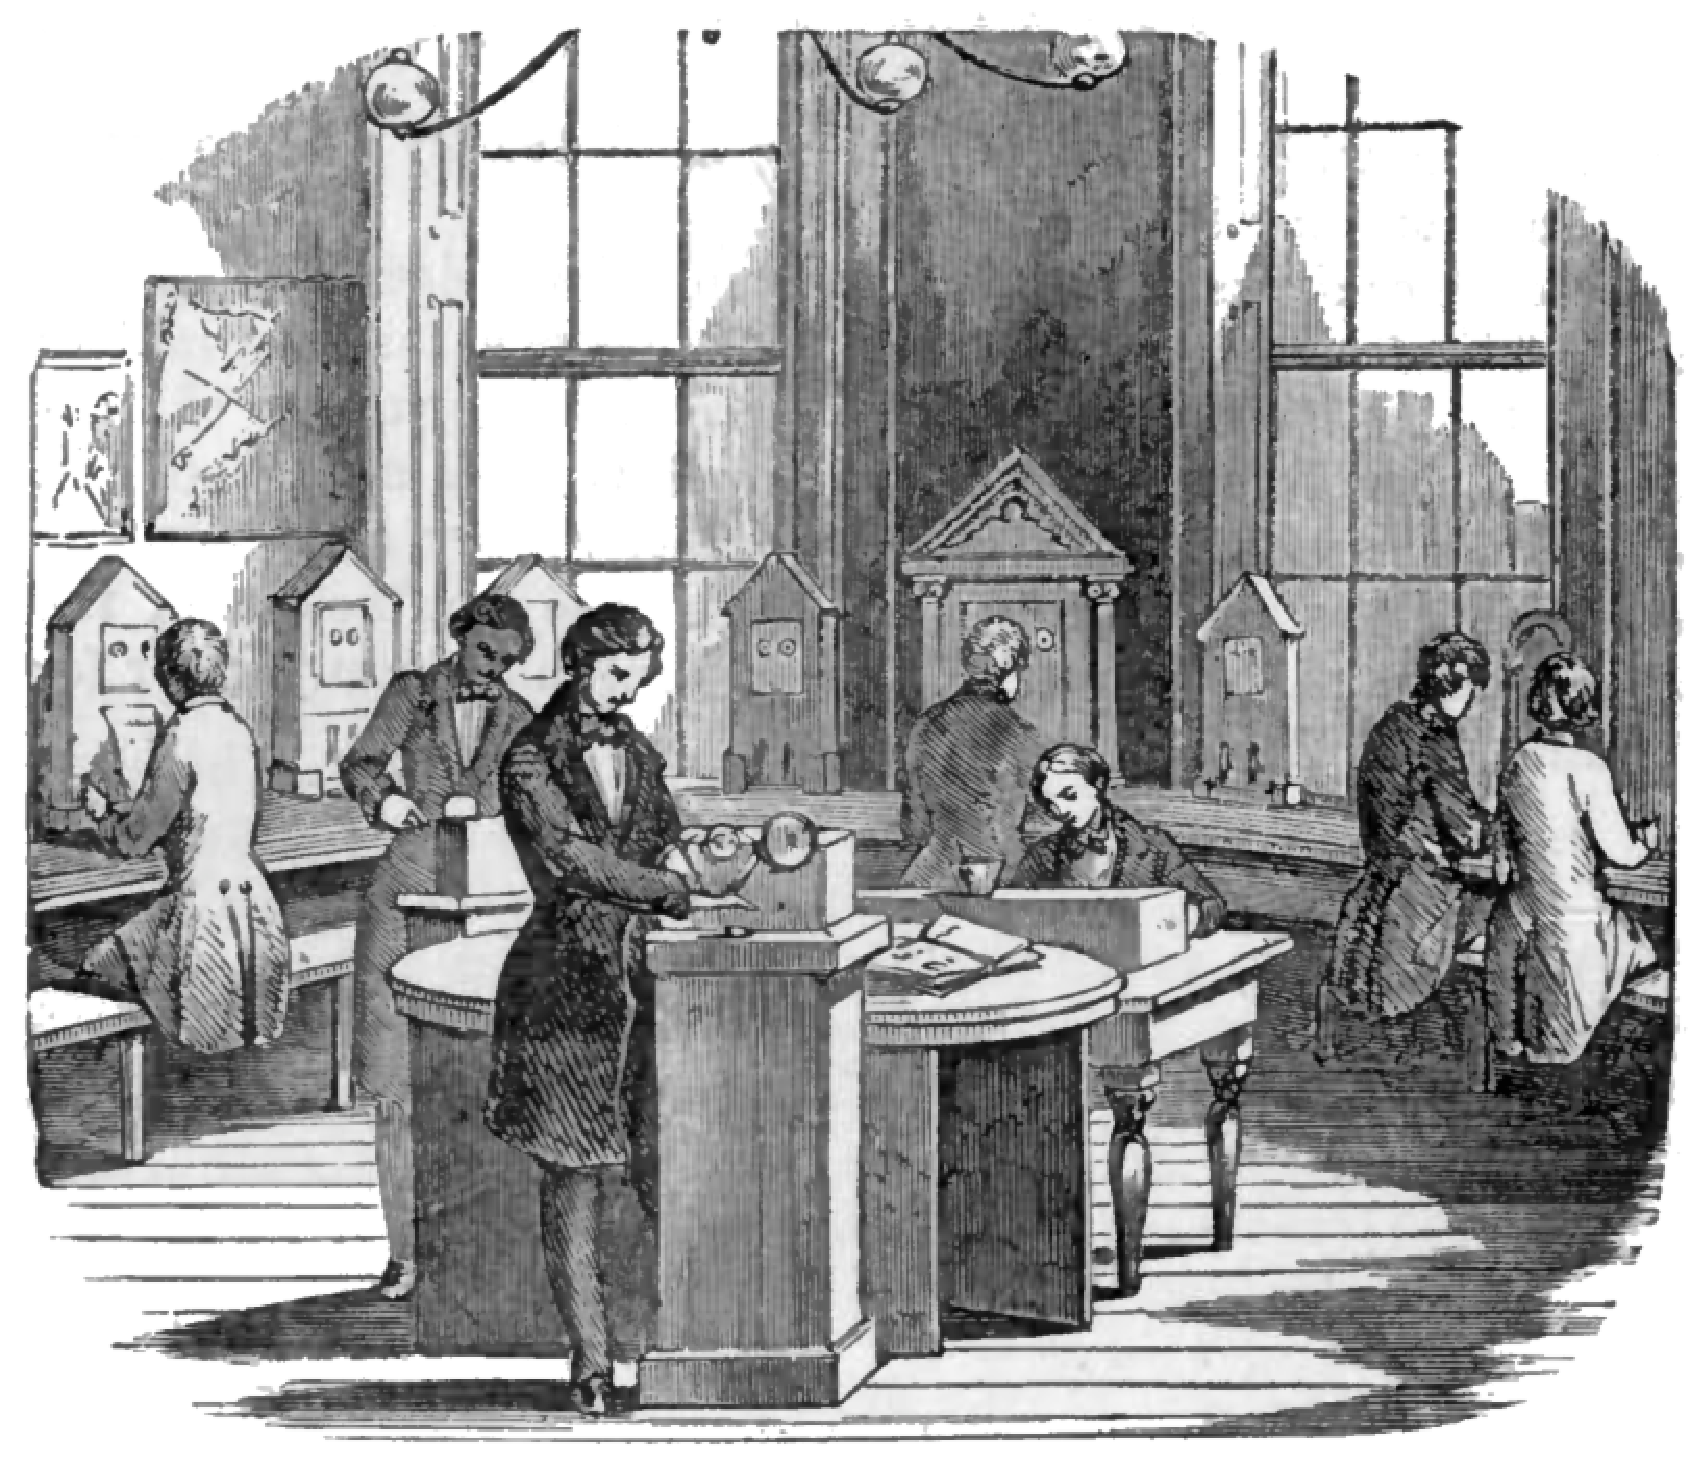
\includegraphics[width=0.8\textwidth]{fig09.pdf}
			\caption*{\small Fonte: \textcite{lardner1867}.}
			\label{fig:308}
		\end{figure}
		
	O código para inserção da figura \ref{fig:308} é mostrado no quadro \ref{cod:fig308}. Códigos também são considerados ilustrações e, caso apresentados, devem apresentar legenda e fonte. $\Rightarrow$ Busque testar o posicionamento delas na folha por meio dos parâmetros b (bottom),t (top),p (page) ou alguma combinação entre eles.
	%
\begin{lstlisting}[caption={Exemplo de inserção de código.}, label={cod:fig308}]
\begin{figure}[ht] % Outras opções: b (bottom),t (top),p (page) ou alguma combinação entre elas
	\centering \label{fig:308}
	\caption{Escritório de telegrafia do século XIX.}
	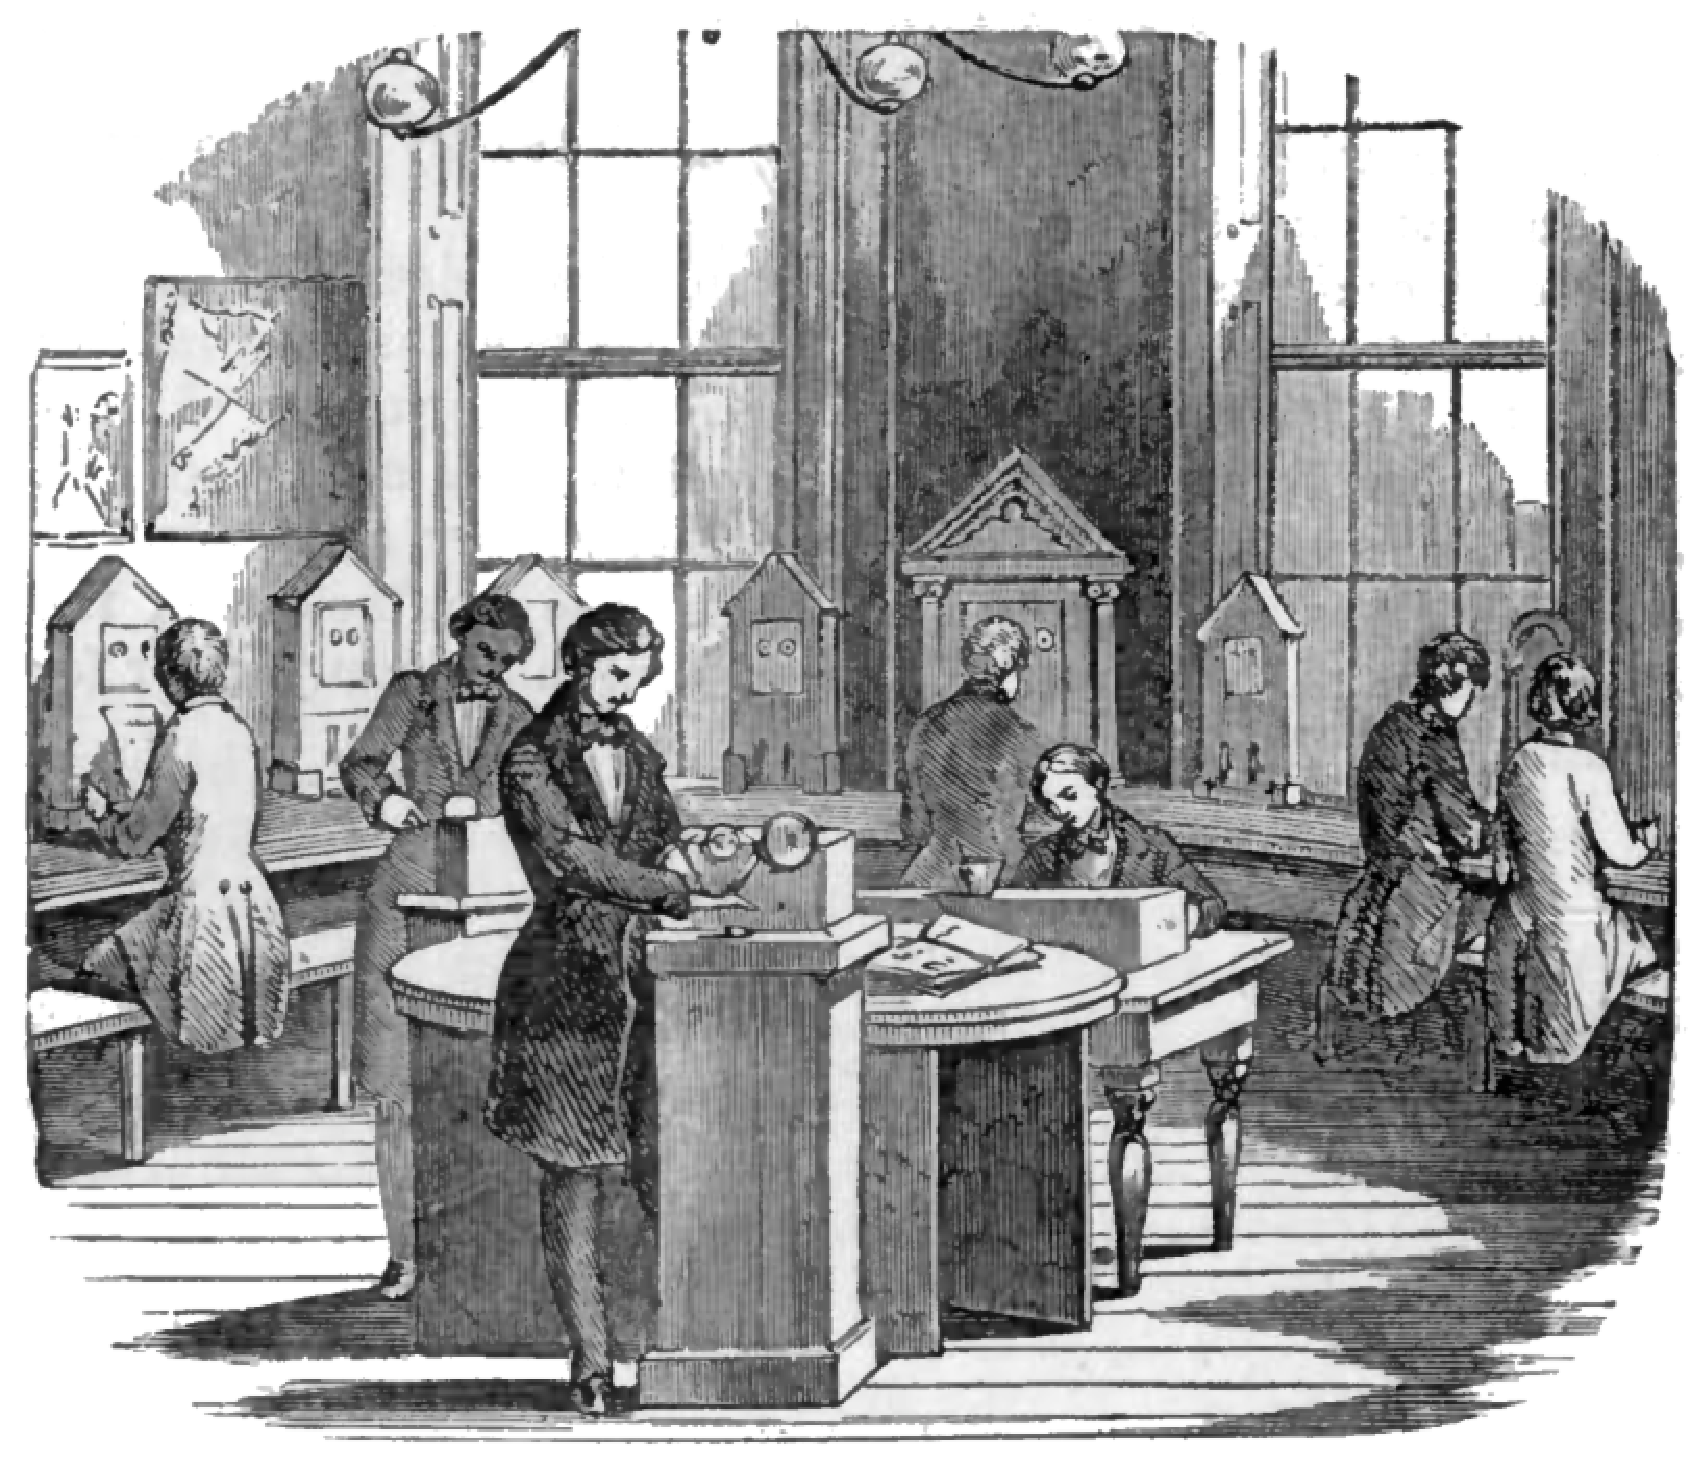
\includegraphics[width=0.7\textwidth]{fig09.pdf}
	\caption*{\small Fonte: \textcite{thomson_1869}.}
\end{figure}
\end{lstlisting}
		
	Para realizar uma referência cruzada da ilustração, isto é, para referenciar algum a página de algum elemento, basta usar o comando \verb*|\pageref{apelido}|, em que o apelido é o termo utilizado, dentro do ambiente para o elemento, com o comando \verb*|\label{apelido}|. Por exemplo, a próxima figura está na página \verb*|\pageref{fig:309}| gera o número de página \pageref{fig:309}. Neste exemplo, o apelido é \verb*|fig:309|, que foi declarado dentro do ambiente da figura. Caso se deseje citar o número do ambiente do elemento desejado (seja ele uma seção, capítulo, nota de rodapé, ilustração ou qualquer outro), ao invés de sua posição no texto, use o comando \verb*|\ref{apelido}|. Experimente alterar a figura de lugar e veja o que acontece!
		
	% figura
	\begin{figure}[ht]
		\centering
		\caption{Linha férrea.}
		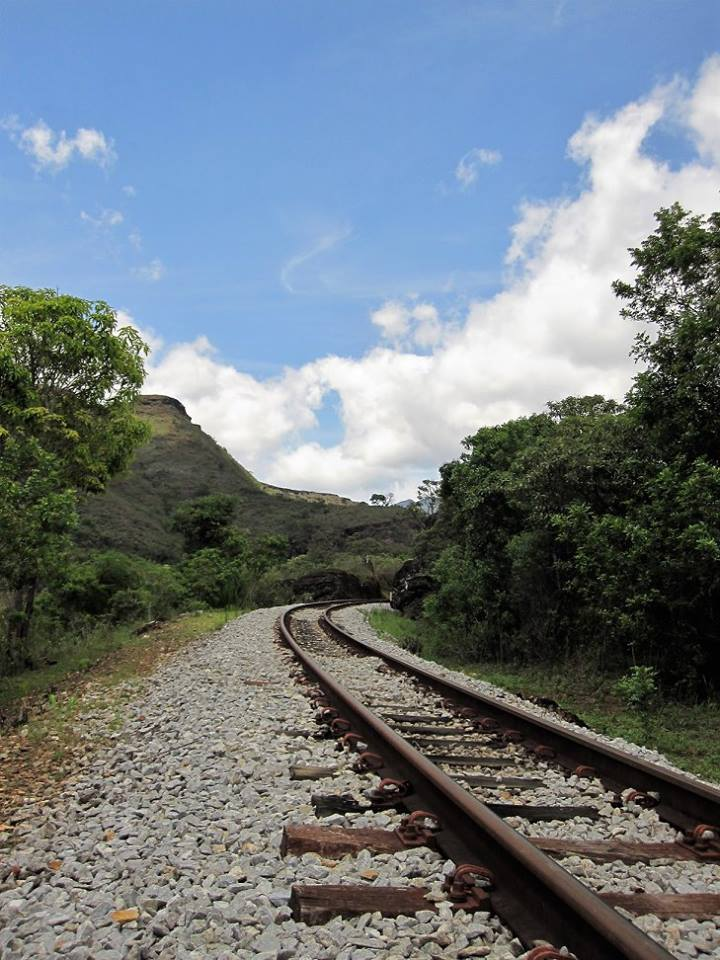
\includegraphics[width=0.5\textwidth]{trem} % teste os valores
		\caption*{\small Fonte: Elaborado pelo autor.}
		\label{fig:309}
	\end{figure}
	 
	$\Rightarrow$ \textbf{Lembre-se:} \textbf{\textcolor{VinhoUFOP}{ Quando o autor do trabalho é o autor da ilustração, a fonte deve ser igualmente citada!}}.

\section{Tabelas}

\subsection{Tabela elaborada em planilha eletrônica}
	Você pode elaborar sua tabela em qualquer planilha eletrônica, como no \verb*|calc|, como ilustra a figura \ref{fig:elaborando-tabela}. No entanto, utilizá-la como uma imagem pode causar problemas de visualização e distorção. Caso escolha elaborar a sua tabela dessa maneira, recomenda-se utilizar algum mecanismo de conversão para o \LaTeX. Existem vários conversores online para este fim, como o \url{latextablegenerator.com}
	
	\begin{figure}[h!]
		\centering
		\caption{Elaborando uma tabela em planilha eletrônica convencional.}
		\label{fig:elaborando-tabela}
		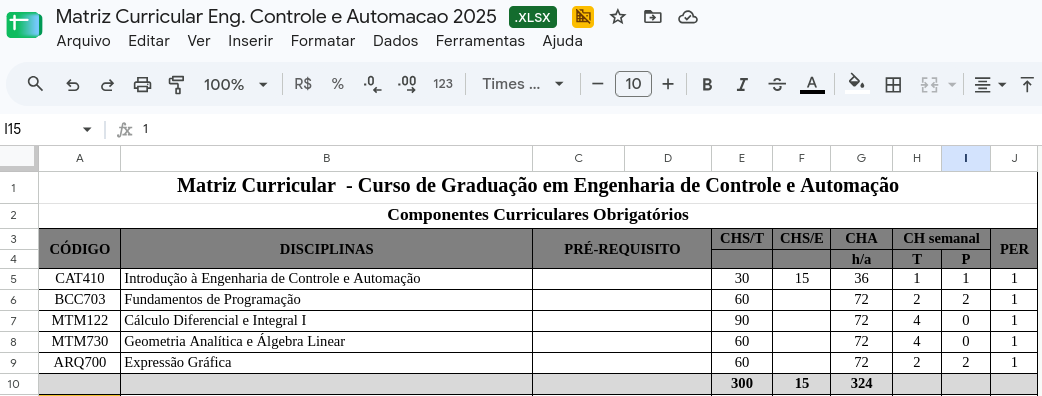
\includegraphics[width=0.8\linewidth]{elaborando-tabela}
		\caption*{\small Fonte: Elaborado pelo autor.}
	\end{figure}
	
	No ambiente de um conversor como ele, há a possibilidade de criar diretamente a tabela, com diversos recursos. O código para gerar a tabela em \LaTeX pode ser obtido clicando-se no botão \emph{generate}, conforme ilustrado na figura \ref{fig:elaborando-tabela2}. 
	
	\begin{figure}[ht]
		\centering
		\caption{Elaborando tabela em um conversor online.}
		\label{fig:elaborando-tabela2}
		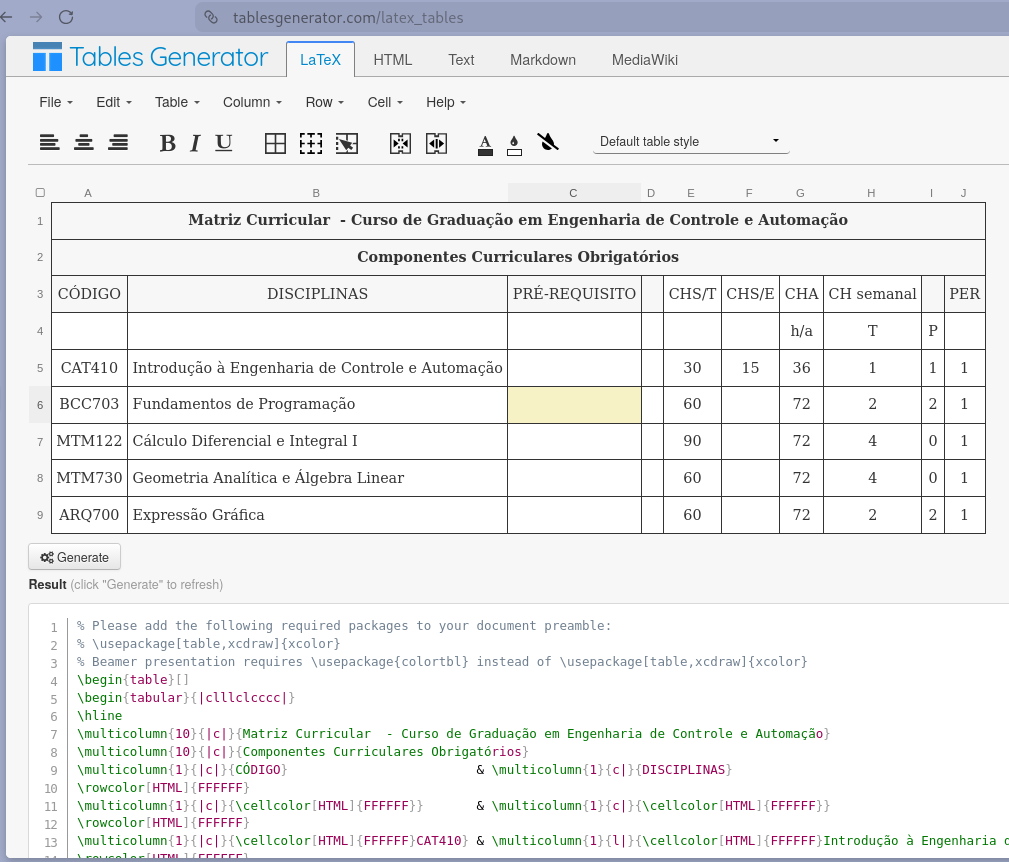
\includegraphics[width=0.8\linewidth]{figuras/elaborando-tabela2}
		\caption*{\small Fonte: Elaborado pelo autor em \url{latextablegenerator.com}.}
	\end{figure}
	
	Agora, caso você não decida manter exatamente a formatação feito em sua  planilha eletrônica, existe também a opção de colar o diretamente da planilha, com a opção  \emph{file/Paste table data}, como ilustrado pela figura \ref{fig:elaborando-tabela3}.
	
	\begin{figure}[ht]
		\centering
		\caption{Utilizando a opção File/Paste table data.}
		\label{fig:elaborando-tabela3}
		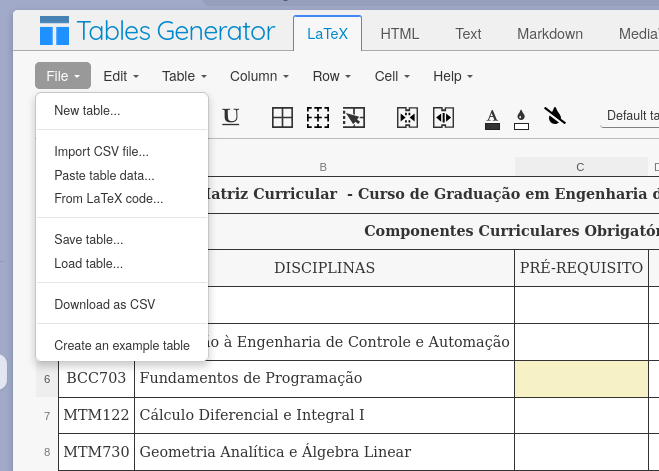
\includegraphics[width=0.8\linewidth]{figuras/elaborando-tabela3}
			\caption*{\small Fonte: \url{latextablegenerator.com}.}
	\end{figure}

\subsection{Tabela elaborada no ambiente table}
	Existem diversas maneiras simples e práticas de se gerar uma tabela bonita e formatada no \LaTeX. A primeira delas é criando a tabela no próprios ambientes \verb*|table| e \verb*|tabular|, exposto na tabela \ref{tab:primeiroP}. Se preferir, use os assistentes em seu editor favorito. 
	% 
	 \begin{table}[b]
	 	\caption{Exemplo de tabela elaborada no ambiente table.}
	 	\label{tab:primeiroP}
	 	\resizebox{\textwidth}{!}{%
	 		\begin{tabular}{||c||c||c||c||c||c||c||c||c||c||}
	 			\hline
	 			\multicolumn{10}{||c||}{Matriz Curricular - Curso de Graduação em Engenharia de Controle e Automação} \\
	 			\hline
	 			\multicolumn{10}{||c||}{Componentes Curriculares Obrigatórios} \\
	 			\hline
	 			CÓDIGO & DISCIPLINAS & PRÉ-REQUISITO &  & CHS/T & CHS/E & CHA & CH semanal &  & PER \\
	 			\hline
	 			&  &  &  &  &  & h/a & T & P &  \\
	 			\hline
	 			CAT410 & Introdução à Engenharia de Controle e Automação &  &  & 30 & 15 & 36 & 1 & 1 & 1 \\
	 			\hline
	 			BCC703 & Fundamentos de Programação &  &  & 60 &  & 72 & 2 & 2 & 1 \\
	 			\hline
	 			MTM122 & Cálculo Diferencial e Integral I &  &  & 90 &  & 72 & 4 & 0 & 1 \\
	 			\hline
	 			MTM730 & Geometria Analítica e Álgebra Linear &  &  & 60 &  & 72 & 4 & 0 & 1 \\
	 			\hline
	 			ARQ700 & Expressão Gráfica &  &  & 60 &  & 72 & 2 & 2 & 1 \\
	 			\hline
	 			&  &  &  & 300 & 15 & 324 &  &  &  \\
	 			\hline
	 		\end{tabular}
	 	}
	 	\caption*{\small Elaborada pelo autor.}
	 \end{table}
 
% --- Seção de Desenvolvimento
\chapter{Desenvolvimento} \label{cap:desenvolvimento}  

\section{Proposição}
	Apresente aqui a afirmação ou ideia central a ser perseguida ao longo do desenvolvimento, em forma de proposição. Ela será, de certa forma, uma possível resposta que poderá conduzir a investigação, constituindo-se em um caminho deliberado para a solução. Caso haja também alguma hipótese a ser testada, ela poderá ser apresentada nas justificativas (no início do texto).
\section{Materiais e Métodos}
	A metodologia é definida como o \textbf{conjunto de métodos ou caminhos} percorridos na busca do conhecimento. O objetivo principal desta seção é fornecer uma \textbf{descrição completa e clara} das principais técnicas, aparatos experimentais e processos empregados durante o desenvolvimento do trabalho. Deve-se distinguir entre o conjunto de procedimentos utilizados para a investigação de fenômenos (métodos de abordagem) e aqueles de caráter mais específico, adequados a cada área de pesquisa (métodos de procedimento).

	\subsection{Tipos de pesquisa}
	 	Envolve a forma de abordagem do problema, a estratégia geral do trabalho, isto é, lida com \textbf{o quê}. Isto é, dependendo da natureza do trabalho, pode-se descrever diferentes modalidades gerais, tais como pesquisa bibliográfica, documental, experimental, de campo, exploratória, descritiva, explicativa, qualitativa, quantitativa, entre outras.
	\subsection{Procedimento metodológico}	
		Tem a ver com \textbf{``como''} o problema será resolvido, o caminho lógico para respondê-lo. Neste caso, as etapas a serem desenvolvidas na metodologia dependerão do tipo de pesquisa proposto.
	\subsection{Procedimentos técnicos}
		Define a técnica de coleta de dados e a descrição, em detalhes, de quais instrumentos serão utilizados na obtenção das informações. Isto é, tem a ver \textbf{com o quê}? É a parte prática e operacional do trabalho em si, e explica a escolha do universo, da amostra, por assim dizer, e das etapas da pesquisa. Alguns exemplos de procedimentos técnicos são:
	\begin{itemize}
		\item[a)] \textbf{Pesquisa Bibliográfica:} Define basicamente uma pesquisa na literatura científica disponível. Por exemplo, ``Uma análise sobre a evolução do conceito de inteligência artificial na educação de 2020 a 2026''. 
		\item[b)] \textbf{Pesquisa Experimental:} É onde se determinam variáveis de influência e formas de controle de efeitos no objeto. Neste caso, é necessário também definir um delineamento Experimental, isto é, será preciso detalhar o planejamento dos testes e a estrutura do experimento. Em geral, é onde se concentram boa parte dos trabalhos de engenharia. 
		\item[c)] \textbf{Pesquisa qualitativa:} Envolve o estudo mais aprofundado de poucos objetos para um conhecimento detalhado.
		\item[d)] \textbf{Estudo de Caso:} Envolve o estudo mais aprofundado de poucos objetos para um conhecimento detalhado. Por exemplo, a monografia defendida na UFOP com o título ``\citetitle{nascimento2022breve}'' teve como foco a transição dos primeiros sistemas de automação analógica e sua consequente digitalização a partir da criação de Controlador Lógico Programável (CLP).\footfullcite[Ver em][]{nascimento2022breve} Neste trabalho, foram levantadas algumas hipóteses, que foram testadas a partir do estudo de uma transição semelhante, em uma planta moderna. 
		\item[e)] \textbf{Pesquisa Documental:} Elaborada a partir de materiais sem tratamento analítico prévio. Por exemplo, o trabalho ``\citetitle{tavares2023medicao}'' buscou contextualizar historicamente o surgimento da comercialização de energia elétrica.\footfullcite[Ver em][]{tavares2023medicao}
		\item[f)] \textbf{Levantamento:} Através da interrogação direta de pessoas cujo comportamento se deseja analisar. Por exemplo, ``A representação das mulheres nas eleições estaduais''.
		\item[g)] \textbf{Pesquisa-Ação:} Realizada em associação com a resolução de um problema coletivo e participação cooperativa. Por exemplo, um estudo sobre ``aumento da evasão escolar de alunos do período noturno'', realizado com os professores e estudantes de uma escola específica.
	\end{itemize}

\subsection{IA na pesquisa: como usar e declarar}
A IAG deve ser vista como um assistente de pesquisa que emula funções de apoio, mas não deve gerir a pesquisa sozinha. Isto é, \textbf{autoria é sempre Humana}: o pesquisador deve manter o controle final e supervisionar criticamente todas as saídas geradas.

De acordo com as \emph{Diretrizes Orientadoras da Utilização da Inteligência Artificial na Educação Brasileira}, recentemente aprovadas no Conselho Nacional de Educação, 
 
Se balizarmos a utilização ética da IA na produção de conhecimento científico, ela poderá ser utilizada em algumas etapas da pesquisa, como planejamento inicial, organização de materiais e referências, entre outras. Poderá também 
apoiar questões de acessibilidade, como tradução supervisionada e transcrição de artigos, desde que respeitadas as leis de proteção de dados e direitos autorais.\footfullcite[Para um aprofundamento, ver][]{sampaio2024diretrizes} 

As diretrizes nacionais, em vias de publicação, dividem as aplicações em categorias de risco: baixo, moderado, alto  e incompatível com as finalidades educacionais.  

Por exemplo, ferramentas usadas para organizar materiais ou fazer revisão textual sem efeito sobre o texto final da monografia podem ser consideradas de baixo risco.

Já sistemas que escrevem trechos inteiros de seções ou capítulos são consideradas incompatíveis, pois são atividades que irão interferir diretamente nas avaliações e decisões acadêmicas, como em uma banca de trabalho final.

Dessa forma, o uso de IA deverá ser  declarado quando tiver participação relevante na elaboração da pesquisa, uma vez que a responsabilidade continua sendo do autor do trabalho, jamais da ferramenta de IA. 

No que se refere estritamente à pesquisa, já existe uma portaria CNPq $n^{\circ}$ 2.664/2026, que instituiu a Política de Integridade na Atividade Científica. Nela é informado que o uso de Inteligência Artificial Generativa (IAG) deve ser declarado de forma clara e transparente, especificando a ferramenta e a finalidade em qualquer fase da pesquisa. \textbf{Recomenda-se que a declaração seja feita na seção de materiais e métodos (ou metodologia).}

\subsection*{Como declarar o uso de IAG} 
\caixa{\begin{exemplo}[Declaração de uso de Inteligência Artificial (IAG)] Conforme as diretrizes de ética acadêmica, declara-se que, durante a preparação desta pesquisa, utilizou-se uma ferramenta de \textbf{Inteligência Artificial Generativa} para a estruturação dos tópicos e geração do código LaTeX e correção de ortografia, baseando-se estritamente nas fontes fornecidas. Após a geração, o conteúdo foi revisado, editado e validado pelo autor, que assume total responsabilidade pelo material final.
\end{exemplo}
}

% Resultados
\section{Resultados} \label{cap:resultados}
Neste capítulo é apresentada uma análise dos resultados obtidos no trabalho.

% Discussões dos resultados
\section{Discussões}

% Conclusões e/ou considerações finais
\chapter{Conclusão}

\section{Considerações finais}
As últimas palavras podem ser apresentadas na seção de conclusão ou considerações finais, a depender do tipo de estudo. Ele pode ser numerado ou não. Caso deseje que a seção ou subseção não possua numeração, utilize \verb*|*| apos o comando. Por exemplo, \verb|\section{Ttítulo do capítulo}|.

% Pós-textual
\postextual

% Referências
\printbibliography[title=REFERÊNCIAS]

% Apêndices e anexos
\begin{apendicesenv} % Apêndice - autoria do próprio autor do texto.

% Apêndice A
\chapter{Material de autoria própria} \label{ape:A}
Apêndices são elementos de autoria do próprio autor do texto.
\chapter{Material de autoria própria} \label{ape:B}
Apêndices são elementos de autoria do próprio autor do texto.
\end{apendicesenv}
% ---

% Anexos
\begin{anexosenv}

% Anexo
\chapter{Material que não é de autoria própria} \label{anexo:A}
Anexos são elementos de autorias de outros, que o autor do texto julga interessante apresentar.

% ---
\end{anexosenv}

%% INDICE REMISSIVO
%\printindex

\end{document}